
%----------------------------------------------------------------------------------------
%	PACKAGES AND DOCUMENT CONFIGURATIONS
%----------------------------------------------------------------------------------------

\documentclass{article}

\usepackage[version=3]{mhchem} % Package for chemical equation typesetting
\usepackage{siunitx} % Provides the \SI{}{} and \si{} command for typesetting SI units
\usepackage{graphicx} % Required for the inclusion of images
\usepackage{natbib} % Required to change bibliography style to APA
\usepackage{amsmath} % Required for some math elements 
\usepackage[utf8]{inputenc}
%\usepackage{natbib}
\graphicspath{ {./images/} }
\setlength\parindent{0pt} % Removes all indentation from paragraphs

\renewcommand{\labelenumi}{\alph{enumi}.} % Make numbering in the enumerate environment by letter rather than number (e.g. section 6)

%\usepackage{times} % Uncomment to use the Times New Roman font

%----------------------------------------------------------------------------------------
%	DOCUMENT INFORMATION
%----------------------------------------------------------------------------------------

\title{Arquitectura de Microcontroladores \\ Practica 1A} % Title


\author{Sergio Hernández Reyes} % Author name

\date{\today} % Date for the report

\begin{document}

\maketitle % Insert the title, author and date



%----------------------------------------------------------------------------------------
%	SECTION 1
%----------------------------------------------------------------------------------------
\section{Objectivo}

Conocer el IDE de desarrollo MPLAB así como sus características y su modo de funcionamiento. En esta practica se intentara correr un código base en el lenguaje ensamblador con el fin de ir debuggeando paso a paso su ejecución.



%----------------------------------------------------------------------------------------
%	SECTION 2
%----------------------------------------------------------------------------------------
\section{Desarrollo}
Se instalo MPLAB correctamente, se crea nuevo proyecto utilizando compilador mpasm (v5.86)\\
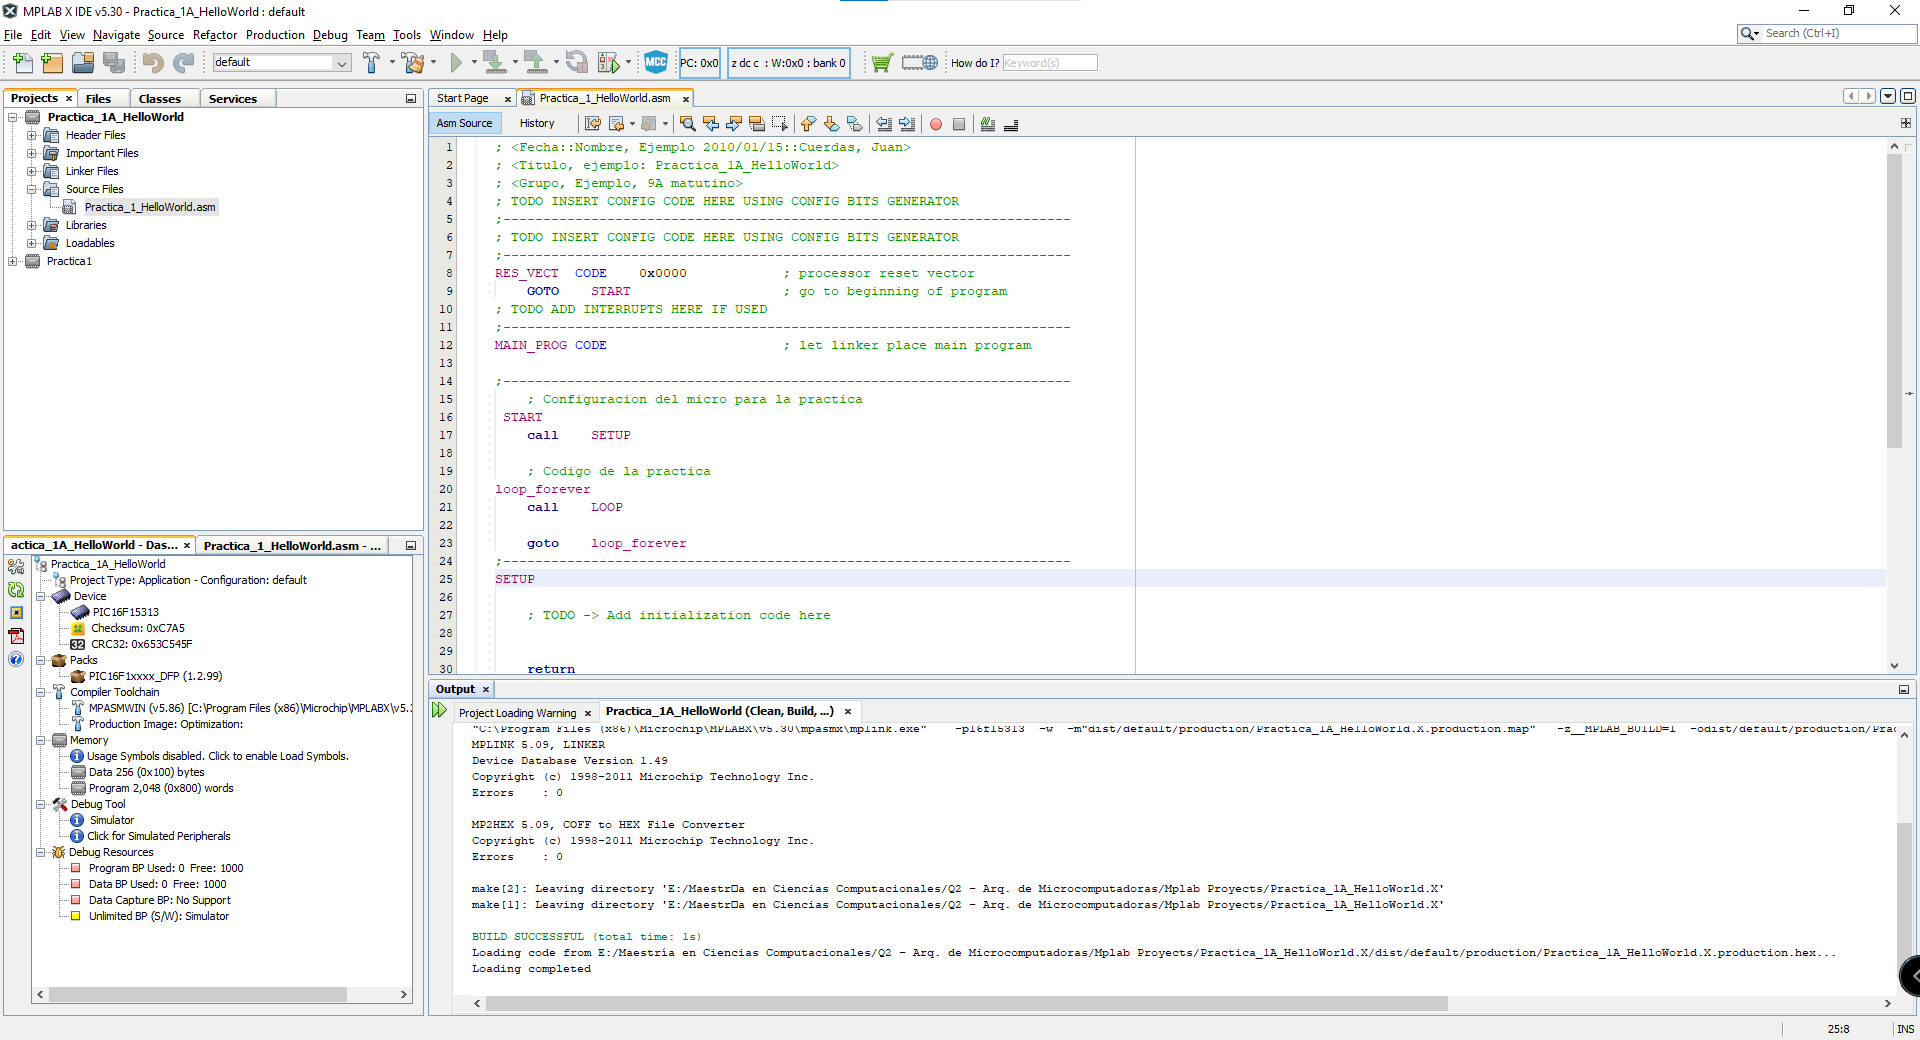
\includegraphics[width=\textwidth]{compilation}\\
Se corre programa con debug habilitado\\
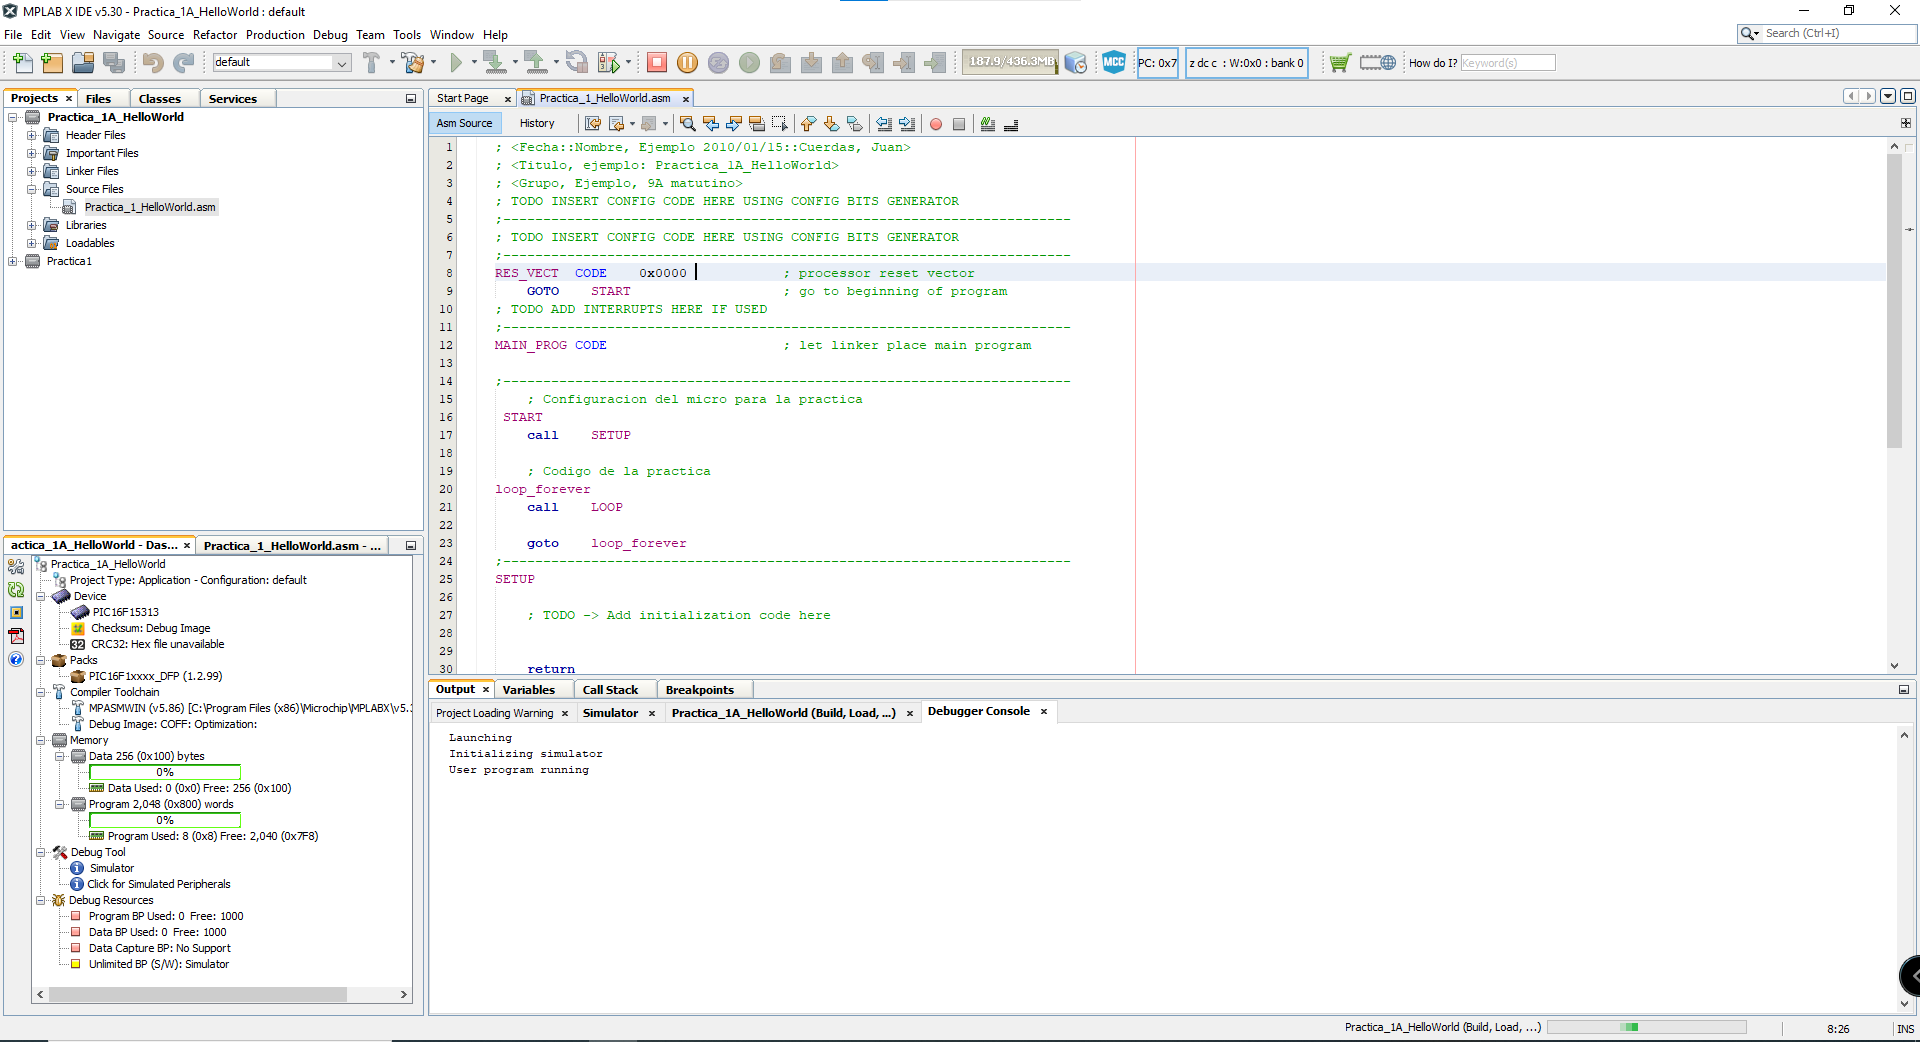
\includegraphics[width=\textwidth]{debug-init}\\
Se pausa ejecución y se avanza siguiente instrucción\\
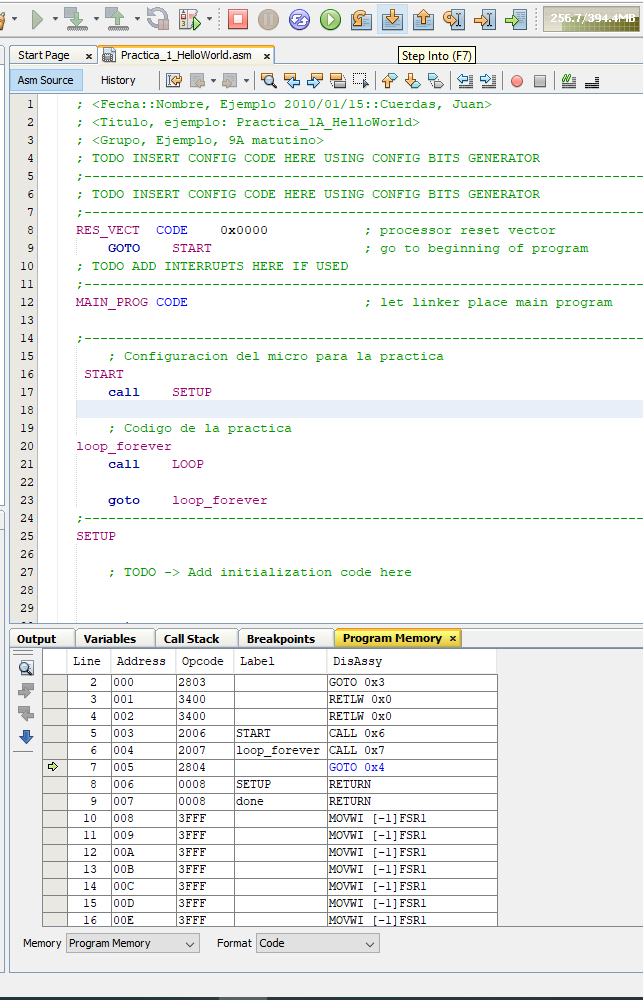
\includegraphics[width=\textwidth]{debug1}\\
Se continua con siguiente instrucción\\
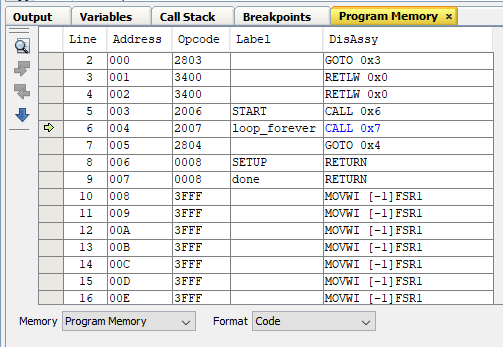
\includegraphics[width=\textwidth]{debug2}\\


%----------------------------------------------------------------------------------------
%	SECTION 3
%----------------------------------------------------------------------------------------
\section{Resultados}
Se corrió la ejecución del programa base obteniendo así un ciclo infinito con el fin de ir debuggeando cada parte del mismo, con el objetivo de familiarizarnos con las herramientas de debuggeo y el IDE en general.



%----------------------------------------------------------------------------------------
%	SECTION 4
%----------------------------------------------------------------------------------------
\section{Conclusiones}
Podemos concluir que nuestro código se ejecuto y está listo para bajarse a nuestro microcontrolador. Que tenemos las herramientas bien configuradas y funcionando en nuestro IDE.

%\begin{figure}[h]
%\begin{center}
%\includegraphics[width=0.65\textwidth]{placeholder} % Include the image placeholder.png
%\caption{Figure caption.}
%\end{center}
%\end{figure}
\end{document}